\documentclass{beamer}
\usepackage[utf8]{inputenc}

\usetheme{Madrid}
\usecolortheme{default}
\usepackage{amsmath,amssymb,amsfonts,amsthm}
\usepackage{txfonts}
\usepackage{tkz-euclide}
\usepackage{listings}
\usepackage{adjustbox}
\usepackage{array}
\usepackage{tabularx}
\usepackage{gvv}
\usepackage{lmodern}
\usepackage{circuitikz}
\usepackage{tikz}
\usepackage{graphicx}

\setbeamertemplate{page number in head/foot}[totalframenumber]

\usepackage{tcolorbox}
\tcbuselibrary{minted,breakable,xparse,skins}



\definecolor{bg}{gray}{0.95}
\DeclareTCBListing{mintedbox}{O{}m!O{}}{%
  breakable=true,
  listing engine=minted,
  listing only,
  minted language=#2,
  minted style=default,
  minted options={%
    linenos,
    gobble=0,
    breaklines=true,
    breakafter=,,
    fontsize=\small,
    numbersep=8pt,
    #1},
  boxsep=0pt,
  left skip=0pt,
  right skip=0pt,
  left=25pt,
  right=0pt,
  top=3pt,
  bottom=3pt,
  arc=5pt,
  leftrule=0pt,
  rightrule=0pt,
  bottomrule=2pt,
  toprule=2pt,
  colback=bg,
  colframe=orange!70,
  enhanced,
  overlay={%
    \begin{tcbclipinterior}
    \fill[orange!20!white] (frame.south west) rectangle ([xshift=20pt]frame.north west);
    \end{tcbclipinterior}},
  #3,
}
\lstset{
    language=C,
    basicstyle=\ttfamily\small,
    keywordstyle=\color{blue},
    stringstyle=\color{orange},
    commentstyle=\color{green!60!black},
    numbers=left,
    numberstyle=\tiny\color{gray},
    breaklines=true,
    showstringspaces=false,
}
\title{4.3.36}
\date{12th September, 2025}
\author{Puni Aditya - EE25BTECH11046}

\begin{document}

\frame{\titlepage}
\begin{frame}{Question}
The line $\vec{r} = \brak{2\hat{i} - 3\hat{j} - \hat{k}} + \lambda\brak{\hat{i} - \hat{j} + 2\hat{k}}$ lies in the plane $\vec{r} \cdot \brak{3\hat{i} + \hat{j} - \hat{k}} + 2 = 0$.
\end{frame}

\begin{frame}{Theoretical Solution}
Let the line L be $\vec{x}$ = $\vec{a}$ + $\lambda\vec{b}$ and the plane P be $\vec{n}^\top\vec{x}$ = $c$ where
\begin{align*}
    \vec{a} = \myvec{2 \\ -3 \\ -1}, \vec{b} = \myvec{1 \\ -1 \\ 2}, \vec{n} = \myvec{3 \\ 1 \\ -1}, \text{c = -2}
\end{align*}
\begin{align}
    \vec{n}^\top\vec{b} &= \myvec{3 & 1 & -1}\myvec{1 \\ -1 \\ 2} \\
    &= \brak{1}\brak{3}+\brak{-1}\brak{1}+\brak{2}\brak{-1} \\
    &= 3-1-2 \\
    \vec{n}^\top\vec{b} &= 0
\end{align}
$\because \vec{n}^\top\vec{b} = 0$, the line L is parallel to plane P.
\end{frame}

\begin{frame}{allowframebreaks}
\frametitle{Theoretical Solution}
\begin{align}
    \vec{n}^\top\vec{a} &= \myvec{3 & 1 & -1}\myvec{2 \\ -3 \\ -1} \\
    &= \brak{2}\brak{3} + \brak{-3}\brak{1} + \brak{-1}\brak{-1} \\
    &= 6-3+1 \\
    &= 4 \neq \text{ c}
\end{align}
$\because \vec{n}^\top\vec{a} \neq c$, the point $\vec{a}$ doesn't line in the plane P. Hence, the line L containing $\vec{a}$ also doesn't lie in the plane. \\
The given statement is \textbf{false}.
\end{frame}

\begin{frame}{Plot}
    \begin{figure}
        \centering
        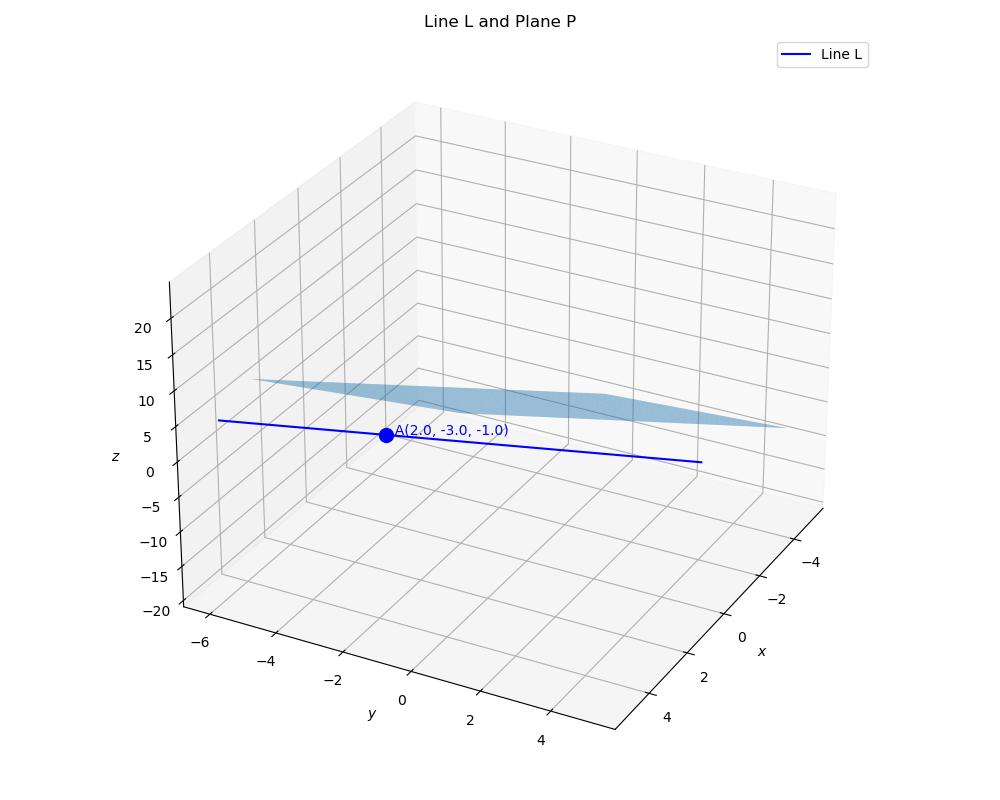
\includegraphics[width=0.7\columnwidth]{../figs/plot_c.jpg}
        \caption{Plot}
        \label{fig:fig}
    \end{figure}
\end{frame}

\end{document}
